% /* cspell:disable */
\documentclass[12pt]{book}

% import package
\usepackage{graphics}   % include graphics
\usepackage{float}      % h!
\usepackage{fancyhdr}
\usepackage{setspace}
\usepackage{sectsty}
\usepackage{amssymb}
\usepackage{amsmath}

% fancyhdr setting
\pagestyle{fancy}
\fancyhead{}
\fancyhead[LO]{\bfseries\rightmark}
\fancyhead[RO]{}
\fancyhead[RE]{\bfseries\leftmark}
\fancyhead[LE]{}
% page setting
\doublespacing
\allsectionsfont{\singlespacing}
\raggedbottom
% math symbols
\DeclareMathOperator*{\argmin}{arg\,min}
\DeclareMathOperator*{\argmax}{arg\,max}

\begin{document}
\tableofcontents

%!TEX root = ../thesis.tex

\chapter{Introduction}

\section{Computational mechanics in civil engineering}

    \subsection{Mathematical model in mechanics}

    \subsection{Numerical method}

    \subsection{Computational mechanics in modern age}

\section{Current difficulties in numerical analysis}

    \subsection{Human effort on meshing}

    \subsection{Imperfection in geometric representation}

    \subsection{Lack of re-meshing scheme}

\section{Proposed approach}

\section{Research contribution}
    
    \subsection{Meshing based on CAD output in 2D and 3D}

    \subsection{High quality elements by Quad-tree}

    \subsection{Auto re-meshing based on error}

\section{Objectives and scope}

\section{Organization of the thesis}

\section{List of publications}


    % /* cspell:disable */
    % \begin{figure}[h!]
    %     \scalebox{1}{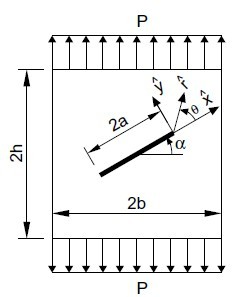
\includegraphics{chapter1/img/crackproblem.jpg}}
    % \end{figure}
    % /* cspell:enabled*/

%!TEX root = ../thesis.tex

\chapter{Literature review}

\section{Overview of numerical methods}

    \subsection{Finite element method}

    \subsection{Boundary element method}

    \subsection{Isogeometric analysis}

\section{Scaled boundary finite element method}

\section{Approaches for meshing automation}

    \subsection{Initial Graphics Exchange Specification (IGES) file}

    \subsection{Non-Uniform Rational B-Spline (NURBS)}

\section{Conclusions}
%!TEX root = ../thesis.tex

\chapter{Isogeometric enhanced scaled boundary finite element method in 2D}

\section{Introduction}

\section{2D NURBS curves}

    \subsection{Shape functions}

    \subsection{Numerical integrations}

\section{Formulation of SBFEM}

    \subsection{Coordinate system}

    \subsection{Displacement function}

    \subsection{Evaluation of the generalized stress intensity factors}

    \subsection{Equation of dynamics}

\section{NURBS enhanced SBFEM}

\section{Numerical examples}

\section{Conclusions}
%!TEX root = ../thesis.tex

\chapter{Quad-tree mesh and auto refinement in 2D analysis based on error}

\section{Introduction}

\section{CAD output in 2D}

\section{NURBS utilization}

    \subsection{Distance function}

    \subsection{Finding intersections}

    \subsection{Optimization}

\section{Quad-tree structure}

\section{Conclusions}
%!TEX root = ../thesis.tex

\chapter{Adaptivity}

\section{Introduction}

\section{Lambda error indicator in SBFEM}

\section{Artificial neural network}

    \subsection{Learning algorithms}

    \subsection{Optimization algorithms}

        \subsubsection{Quasi-Newton methods}

        \subsubsection{Stochastic gradient descent}

        \subsubsection{Stochastic gradient-based optimizer proposed by Kingma, Diederik, and Jimmy Ba}

    \subsection{Activation function}

        \subsubsection{Identity}

        \subsubsection{Logistic}

        \subsubsection{Tanh}

        \subsubsection{Rectified linear unit function}

    \subsection{Learning rate}

    \subsection{Backpropagation algorithm}

\section{Multi-layer perceptron}

\section{Conventional neural network(not decided yet)}

\section{Numerical examples}

\section{Conclusions}


%!TEX root = ../thesis.tex

\chapter{Isogeometric enhanced SBFEM in 3D}

\section{Introduction}

\section{Formulation of SBFEM in 3D}

\section{CAD output in 3D}

\section{NURBS in 3D}

    \subsection{Surfaces division}

    \subsection{Finding projection}

    \subsection{Optimization using matrix representation}

\section{Numerical examples}

\section{Conclusions}
%!TEX root = ../thesis.tex

\chapter{Conclusions and recommendation}

% /* cspell:enabled*/




































\end{document}